\chapter{Methodology}
\label{ch:methods}

\section{Overview of the Proposed Method}

The proposed method aims to address the problem of h-index inflation by
developing two novel metrics that adjusts for the subject area and the quality
of the journal in which the publication is published. The first metric, the
\textit{Adjusted h-index} ($h_{\text{adj}}$), adjusts the h-index by only
considering publications from the top 20\% of journals in it's corresponding
subject area, based on the h5 index of the journal. The second metric, the
\textit{JIF-adjusted h-index} ($h_{\text{JIF}}$), adjusts the h-index
similarly, but the ranking of the journals is determined by the Journal Impact
Factor (JIF) of the journal in which the publication is published. The proposed
method is implemented in \emph{SQL} and the data is stored in a Sqlite
database.

\section{Data Collection and Preprocessing}

For the purpose of this study, the Alexandria3k \cite{Spi23g} tool was used to
collect publication data from the Crossref Dataset \cite{Crossref2020} and
prepare the data for processing. Alexandria3k supplies a library and a
command-line tool providing efficient relational query access to diverse
publication open data sets. Specifically, the dataset that was used is a subset
of the Crossref-2024 and Crossref-2023 datasets, which contain publication
metadata from about 156 million publications from all major international
publishers with full citation data for around 60 million of them. In addition
to that, for the subject of the publications, the Scopus ASJC (All Science
Journal Classification) subject codes were used.

To be more specific, the ASJC codes were used to categorize the publications
into more general subject areas than the original subject areas provided by the
Crossref-2023 dataset. The ASJC codes are a standard classification system used
to categorize publications into subject areas and are widely used in the
scientific community. The ASJC codes are hierarchical and are organized into
four levels, with the first level being the broadest and the fourth level being
the most specific. For the purpose of this study, the first level of the ASJC
codes was used to categorize the publications into subject areas. Crucial to
note is that the ASJC codes are not available for all publications in the
Crossref-2024 dataset \cite{crossrefSubjectCodes2024}, so only journals with
subjects from the Crossref-2023 dataset were considered for this study, since
for those journals the ASJC codes were able to be retrieved.

\section{Implementation of the Proposed Methods}
%
%The proposed method was implemented in SQL using the Sqlite database management
%system. The implementation consists of two main parts: the calculation of the
%Adjusted h-index and the calculation of the JIF-adjusted h-index based on the
%last 3 years. The implementation of the Adjusted h-index is done in these
%steps: (1) Create tables to store and index works and authors (2) Create a
%common table for journals by issn along with their general subject area (3)
%Count citations for Each Work (4) Calculate the h3 index of the journals (5)
%Identify the top 20\% of journals by subject based on H3 index (6) Create
%filtered works tables from the top Journals by Subject (7) Calculate the
%average h3 index for each subject area (8) Calculate the Adjusted h-index for
%each author
%
%Similarly, the implementation of the JIF-adjusted h-index is done in these
%steps: (1) Calculate Work Citations (2) Filter Citable Works (3) Calculate
%Number of Publications in the Impact Factor Period (4) Calculate the Journal
%Impact Factor (JIF) (5) Identify the top 20\% of journals by subject based on
%H3 index (6) Create filtered works tables from the top Journals by Subject (7)
%Calculate Average h-index by Subject (8) Calculate Adjusted h-index
%
%\section{Implementation of the Proposed Method}
%

The proposed method was implemented in SQL using the SQLite database management
system. The implementation consists of two main parts: the calculation of the
Adjusted h-index and the calculation of the JIF-adjusted h-index based on the
last 5 years, specifically the last 3 for the Impact Factor calculation. Both
methods share the same structure and preparation steps, with the main
difference being the metrics (H5 and IF3) used to rank the journals. In order
to use the subject codes from the Scopus ASJC classification, since they are
not available in the Crossref-2024 dataset, the journals (ISSN) along with
their subject codes were extracted from the Crossref-2023 dataset and stored in
a separate table. Additionally, if the ASJC codes were not available for a
journal, even from the Crossref-2023 dataset, the Scopus API was used to
retrieve the subject codes, if possible. After that, the preparation of the
database involves creating tables to store and index works and authors, as well
as a common table for journals by ISSN and subject.

\subsection{Calculation of the Adjusted h-index}

%\begin{itemize}
%    \item \textbf{Preparation of the Database}
%          \begin{enumerate}
%              \item \textbf{Create Tables for Works and Authors}: Establish tables to store and index works
%                    and their associated authors using ORCID identifiers. This ensures that each work is linked to its respective authors.
%
%              \item \textbf{Create Common Table for Journals by ISSN and Subject}: Create a table that consolidates journal
%                    entries by their ISSN along with their general subject area, ensuring that each work is correctly categorized.
%          \end{enumerate}
%\end{itemize}
\begin{enumerate}
      \item \textbf{Count Citations for Each Work}: Calculate the number of citations for each work to determine its impact.

      \item \textbf{Calculate the h5 Index of Journals}: Derive the h5 index for journals, which is a
            measure of their citation impact over the past three years.

      \item \textbf{Identify the Top 20\% of Journals by Subject Based on h5 Index}: Determine the top 20\% of journals within
            each subject area based on their h5 index.

      \item \textbf{Create Filtered Works Tables from the Top Journals by Subject}: Generate tables that include works from the
            top journals for each subject area, ensuring that only high-impact works are considered.

            %\item \textbf{Calculate the Average h5 Index for Each Subject Area}: Compute the average h3 index for each subject area
            %      to provide a benchmark for comparison.

      \item \textbf{Calculate the Adjusted h-index for Each Author}: Determine the adjusted h-index for each author,
            taking into account the subject area of the author.
\end{enumerate}

\subsection{Calculation of the JIF-adjusted h-index}
\begin{enumerate}
      \item \textbf{Calculate Work Citations}: Compute the number of citations for each work to assess their impact.

      \item \textbf{Filter Citable Works}: Identify works that are longer than two pages to exclude non-research articles such as news or book reviews.

      \item \textbf{Calculate Number of Publications in the Impact Factor (IF) Period}: Count the number of publications
            for each journal within the IF period (last 3 years).

      \item \textbf{Calculate the Journal Impact Factor (JIF)}: Derive the JIF by dividing the number of citations by
            the number of publications for each journal.

      \item \textbf{Identify the Top 20\% of Journals by Subject Based on JIF}: Select the top 20\% of journals within
            each subject area based on their JIF\@.

      \item \textbf{Create Filtered Works Tables from the Top Journals by Subject}: Generate tables that include works from
            the top journals for each subject area, ensuring that only high-impact works are considered.

            %\item \textbf{Calculate the Average h-index for Each Subject Area}: Compute the average h-index for each subject area to
            %      provide a benchmark for comparison.

      \item \textbf{Calculate the Adjusted h-index for Each Author}: Determine the adjusted h-index for each author.
\end{enumerate}

\section{ROLAP Analysis}

The proposed method was implemented using a Relational Online Analytical
Processing (ROLAP) approach. ROLAP is a database management system that enables
users to analyze multidimensional data stored in a relational database
\cite{codd1993providing}. The implementation of the proposed method in ROLAP
allows for efficient querying and analysis of the publication data to calculate
the adjusted h-index and JIF-adjusted h-index. For the ROLAP implementation,
the tool Simple-rolap \cite{simple-rolap} was used, which provides a simple
framework for maintainable and time-efficient relational online analytical
processing (ROLAP) by enabling the specification of small, modular SQL queries.
It is designed for querying rarely modified data sets and is particularly
useful in scenarios where materialized views are unsupported or unusable.

The primary function of Simple-ROLAP is to save the result of each SQL query in
corresponding tables, which can then be used by subsequent queries. This
modular approach allows for the independent development and testing of each
query. Automatic dependency analysis ensures that new queries can utilize
already calculated results and that when a query is changed, only the dependent
tables are automatically repopulated.

\section{Testing of the Proposed Method}
For the testing of the proposed methods, the RDBUnit \cite{rdbunit} tool was
used to create and execute unit tests for the SQL queries. RDBUnit is a
database unit testing framework that allows for the creation of test cases for
SQL queries and stored procedures. The tool provides a simple and efficient way
to express the setup prior to a query, the query itself, and the expected
results. This framework can test \texttt{SELECT} queries as well as queries
used for creating tables and views, offering flexibility in how tests are
structured.

RDBUnit enables the embedding of all types of queries directly into the test
script or the inclusion of queries from external files. It streamlines the
creation of input and expected result tables by automatically inferring the
types of the tables' fields, thus reducing the overhead typically associated
with setting up test environments. This makes RDBUnit an ideal choice for
ensuring the accuracy and reliability of SQL queries used in the proposed
methods, enhancing the overall robustness of the data analysis process.

\section{Detailed Calculation of the Adjusted h-indexes}

In detail, for the calculation of the Adjusted h-indexes, the SQL tables are as
follows:

\subsection{Data from Crossref-2024 Dataset}
\begin{itemize}
      \item \textbf{Works}: Contains the works with their respective DOIs and the number of citations.
      \item \textbf{Authors}: Contains the authors with their respective ORCID identifiers.
      \item \textbf{Journals}: Contains the journals with their respective ISSNs and subject areas.
      \item \textbf{ASJC}: Contains the ASJC codes for the subject areas.
      \item \textbf{Work References}: Contains the references of the works.
\end{itemize}

\subsection{ROLAP Analysis Tables}

\noindent\textbf{1: Data Preparation}
\begin{itemize}
      \item \textbf{works\_orcid}: Contains the works with their respective authors.
      \item \textbf{works\_issn\_subject}: Contains the journals with their respective subject areas.
      \item \textbf{work\_citations}: Contains the works with their respective citations.
\end{itemize}

\vspace{1em} % Add space to separate the comment
\noindent\emph{For Impact Factor calculation only:}
\begin{itemize}
      \item \textbf{Citations}: Contains the works that were published in the last year and cited from works published in the last two years.
      \item \textbf{Citable\_Works}: Contains the works that are longer than two pages.
      \item \textbf{Publications}: Contains the number of publications for each journal within the IF period.
\end{itemize}

\noindent\textbf{2: Calculation of Journal h5 Index}
\begin{itemize}
      \item \textbf{issn\_subject\_h5}: Calculates the h5 index of the journals.
\end{itemize}

\noindent\textbf{3: Calculation of Journal Impact Factor (JIF)}
\begin{itemize}
      \item \textbf{impact\_factor}: Calculates the Journal Impact Factor (JIF) for each journal.
\end{itemize}

\noindent\textbf{4: Getting Top and Bottom Percentile of Journals}
\begin{itemize}
      \item \textbf{top\_issn\_by\_subject}: Contains the top 20\% of journals by subject based on the h5 index or JIF.
      \item \textbf{bottom\_issn\_by\_subject}: Contains the bottom 60\% of journals by subject based on the h5 index or JIF.
\end{itemize}

\noindent\textbf{5: Filtered Works Tables}
\begin{itemize}
      \item \textbf{filtered\_works\_orcid}: Contains the works from the top journals by subject.
      \item \textbf{bottom\_filtered\_works\_orcid}: Contains the works from the bottom journals by subject.
\end{itemize}

\noindent\textbf{6: Calculation of the Adjusted h-index}
\begin{itemize}
      \item \textbf{orcid\_h5\_filtered}: Calculates the h5 index for each author.
      \item \textbf{orcid\_h5\_bottom}: Calculates the h5 index for each author from the 'lower quality' journals.
\end{itemize}

Figure \ref{fig:tables} shows the dependencies of each table for the
implementation of the Adjusted h-index by filtering the top 20\% of journals by
subject based on the h5 index.

\begin{figure}[H]
      \centering
      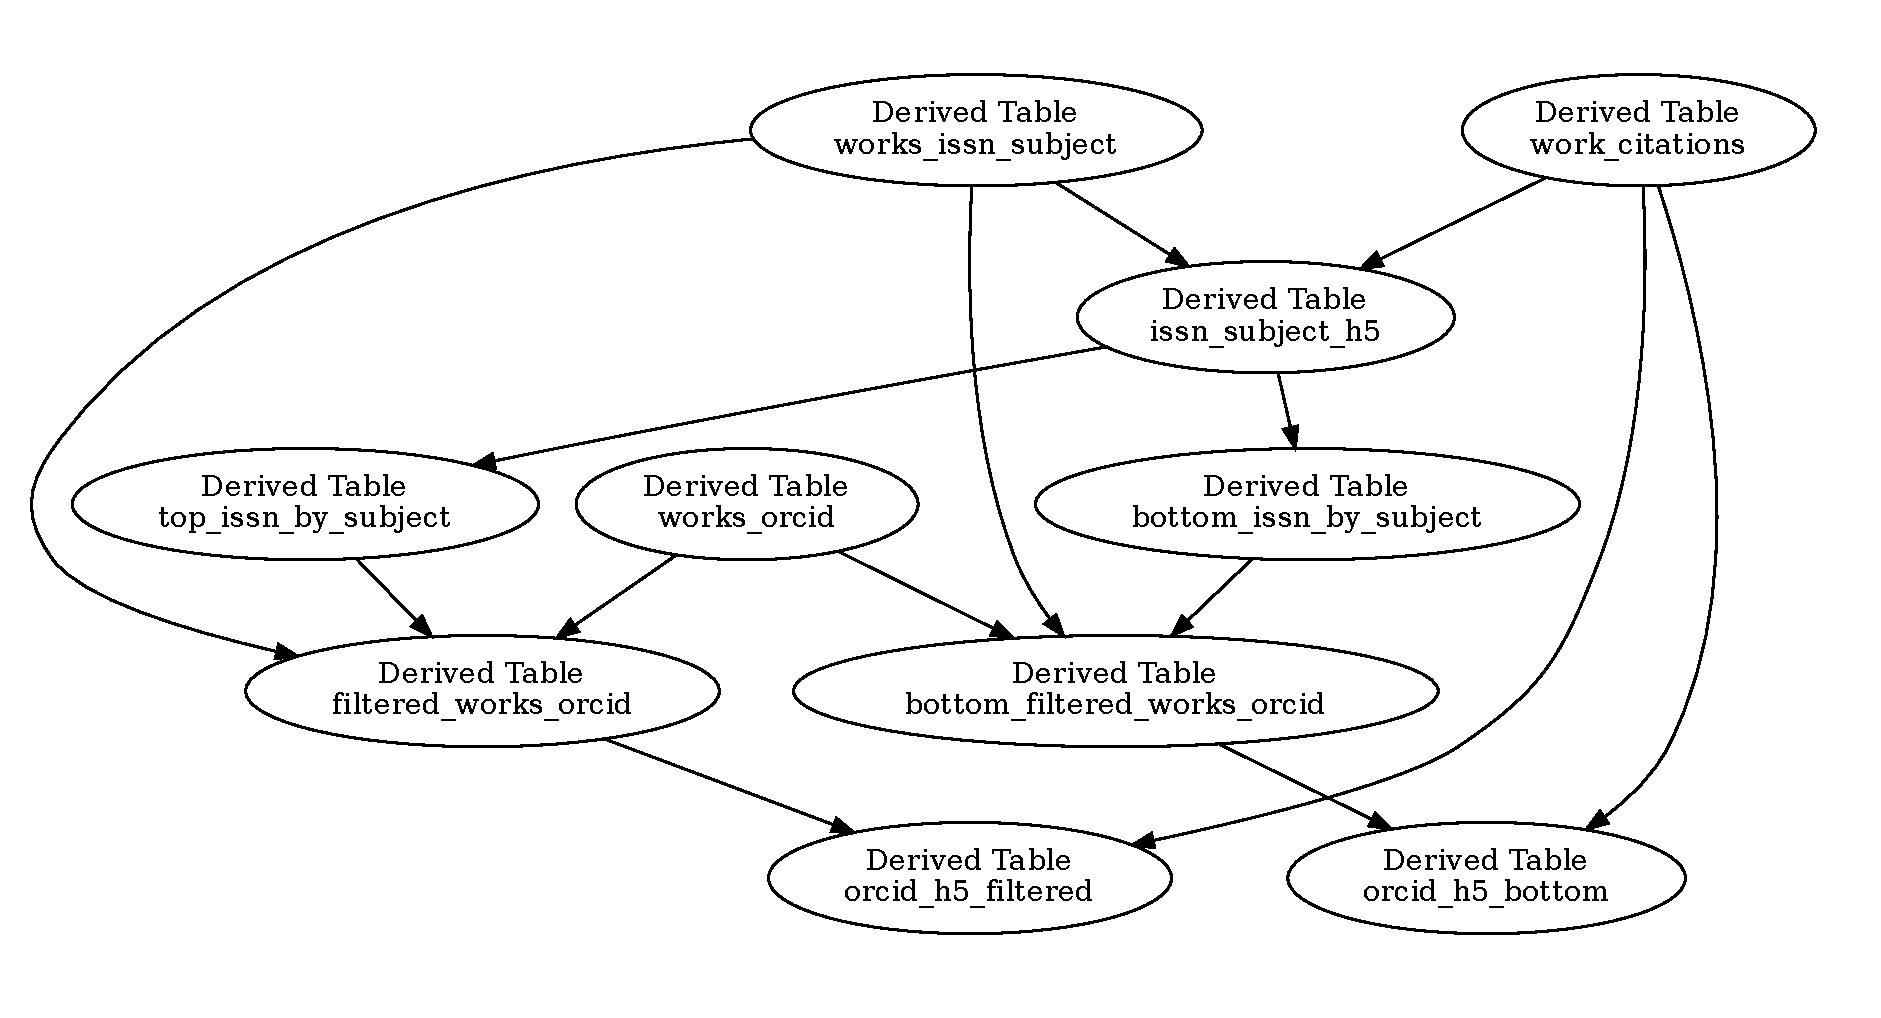
\includegraphics[width=0.8\textwidth]{../figs/h5.pdf}
      \caption{Dependencies of the tables used in the implementation of the Adjusted h-index by filtering the top 20\% of journals by subject based on the h5 index.}
      \label{fig:tables}
\end{figure}

Figure \ref{fig:tables2} shows the dependencies of each table for the
implementation of the JIF-adjusted h-index by filtering the top 20\% of
journals by subject based on the Journal Impact Factor (JIF).

\begin{figure}[H]
      \centering
      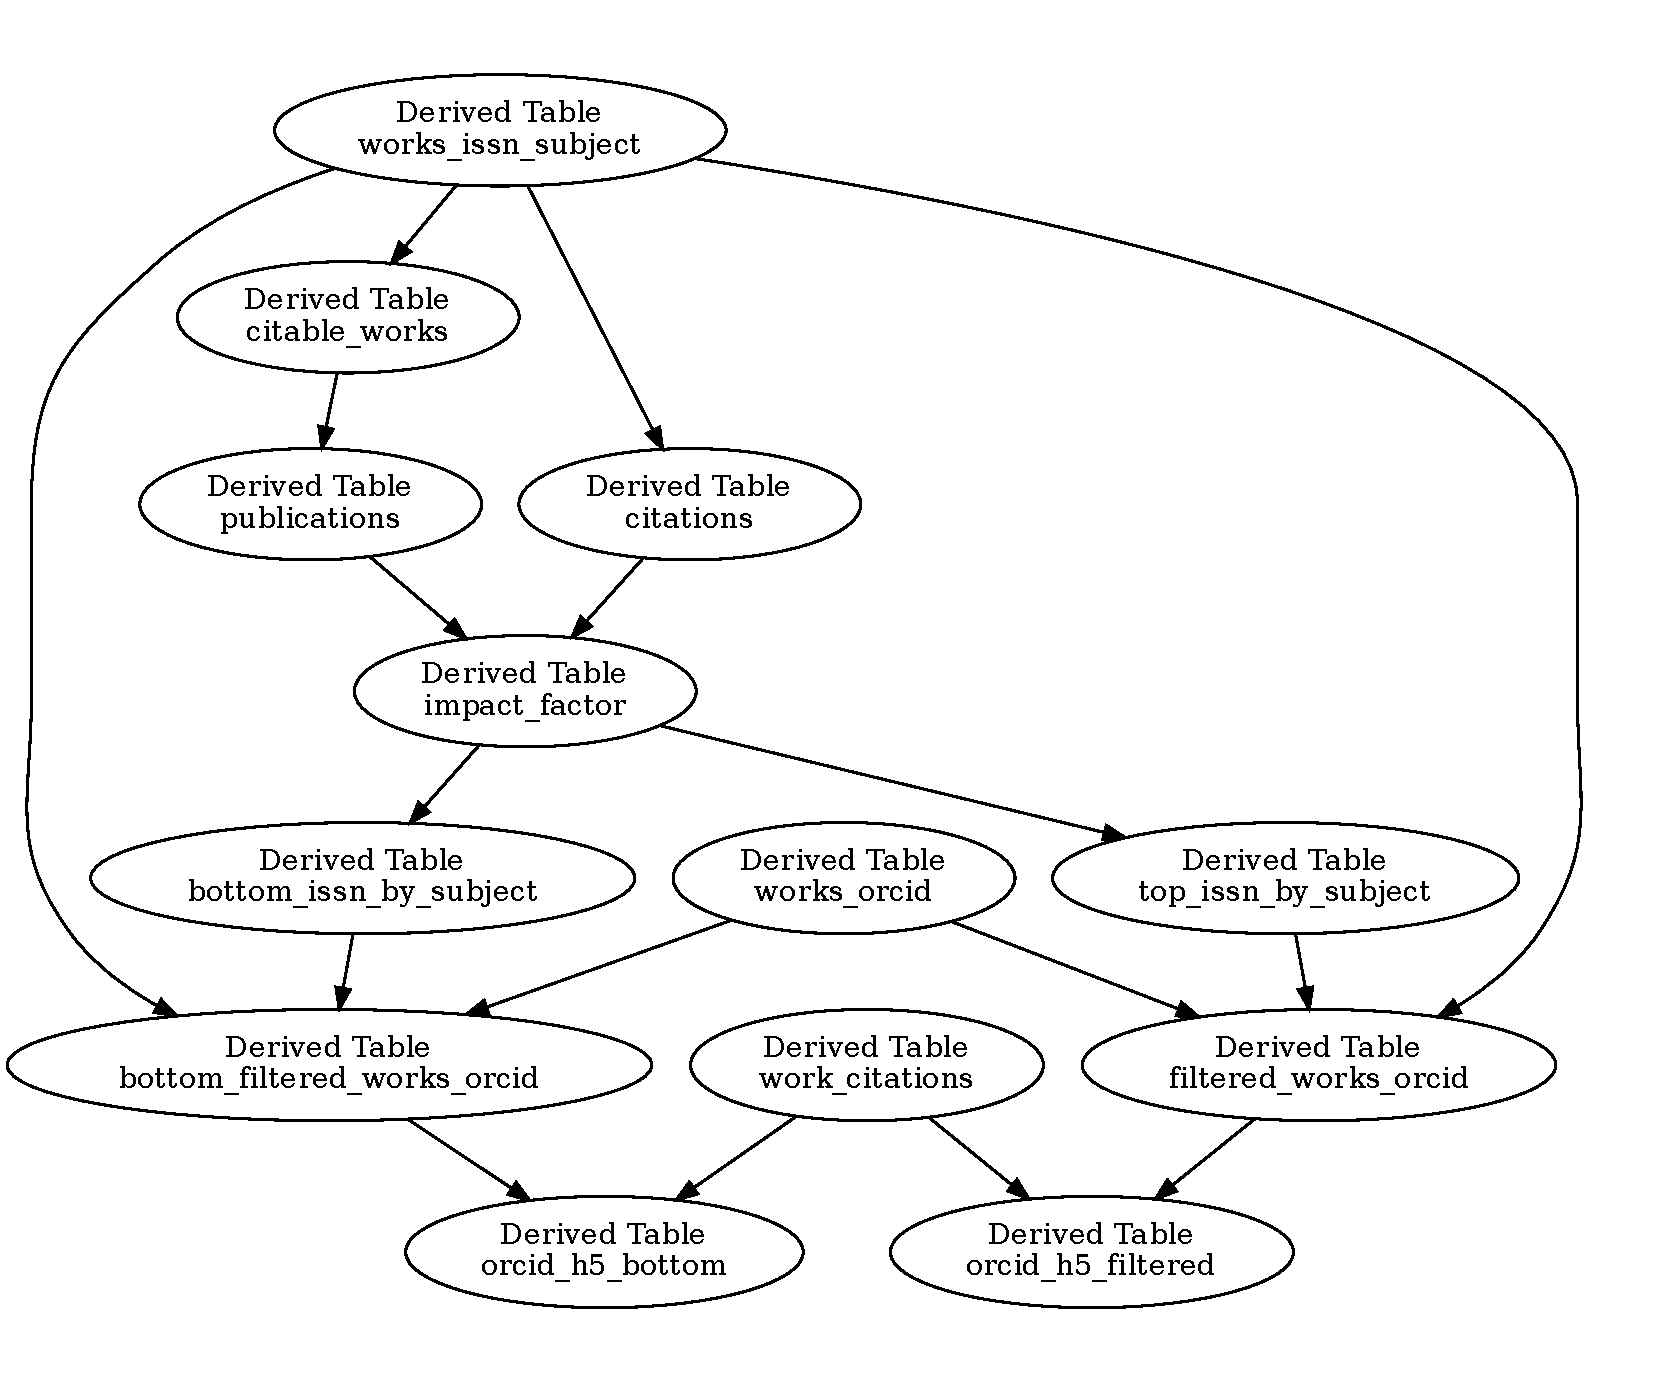
\includegraphics[width=0.8\textwidth]{../figs/impact.pdf}
      \caption{Dependencies of the tables used in the implementation of the JIF-adjusted h-index by filtering the top 20\% of journals by subject based on the Journal Impact Factor (JIF).}
      \label{fig:tables2}
\end{figure}
%Figure \ref{fig:tables} shows the dependencies of each table.
%
%\begin{figure}[H]
%    \centering
%    \includegraphics[width=0.8\textwidth]{figures/tables.png}
%    \caption{Dependencies of the tables used in the calculation of the Adjusted h-indexes.}
%    \label{fig:tables}
%\end{figure}

%Figure \ref{fig:tables} shows the dependencies of each table.
%
%\begin{figure}[H]
%    \centering
%    \includegraphics[width=0.8\textwidth]{figures/tables.png}
%    \caption{Dependencies of the tables used in the calculation of the Adjusted h-indexes.}
%    \label{fig:tables}
%\end{figure}

%Here we can see the dependencies of each table, see Figure \ref{fig:tables}.
%
%\begin{figure}[H]
%      \centering
%      \includegraphics[width=0.8\textwidth]{figures/tables.png}
%      \caption{Dependencies of the tables used in the calculation of the Adjusted h-indexes.}
%      \label{fig:tables}
%\end{figure}
%

--- Methodology involves the design of research developed to test
hypotheses or answer questions developed from the background section. Include
details about data collection methods, analysis techniques, and tools, and
technologies used. In systems-building research in this chapter you might also
include your system's design and architecture.

Be careful regarding terminology: You describe \emph{methods} (not
methodology). This description is termed \emph{methodology}.

Base your methodological presentation using the terms introduced in reference
\cite{SF18}.

